We use numerical simulations to verify our theoretical ROC curve predictions from Section \ref{sec:roc_theory} that rely on RMT approximations presented in Section \ref{sec:rmt}. We also demonstrate properties of the new RMT detectors that we derived in Section \ref{sec:rmt_detecs}, as described next.


\subsection{Simulation Protocol}\label{sec:sim_proto}

To compute an empirical ROC curve, we first generate a random subspace, $U$, by taking the first $k$ left singular vectors of a random matrix with i.i.d. $\mathcal{N}(0,1)$ entries. Using this $U$, we generate training samples as described in Section \ref{sec:training_data} from which we form estimates $\widehat{U}$ and $\widehat{\Sigma}$ from the eigenvalue decomposition of the sample covariance matrix as described in (\ref{eq:param_estims_stoch}).

We then generate a desired number of test samples from each hypothesis using either (\ref{eq:stoch_setup}) or (\ref{eq:determ_setup}). For each test sample, we compute the test statistic for each detector. Using Fawcett's \cite{fawcett2006introduction} `Algorithm 2', we compute an empirical ROC curve by first sorting the test statistics. At each statistic, we log a (PF, PD) pair by counting the number of lower scores generated from each hypothesis. This is repeated for multiple realizations of $U$, generating multiple empirical ROC curves. We refer to a single empirical ROC curve corresponding to a realization of $U$ as a trial. We then average the empirical ROC curves over multiple trials using Fawcett's \cite{fawcett2006introduction} `Algorithm 4'. This performs threshold averaging by first uniformly sampling the sorted list of all test scores of ROC curves and then computing (PF, PD) pairs in the same way as `Algorithm 2'.


\subsection{Convergence and Accuracy of ROC Curve Predictions}
\begin{figure}[t]
\centering
\subfigure[$k=2$, $c=1$]{
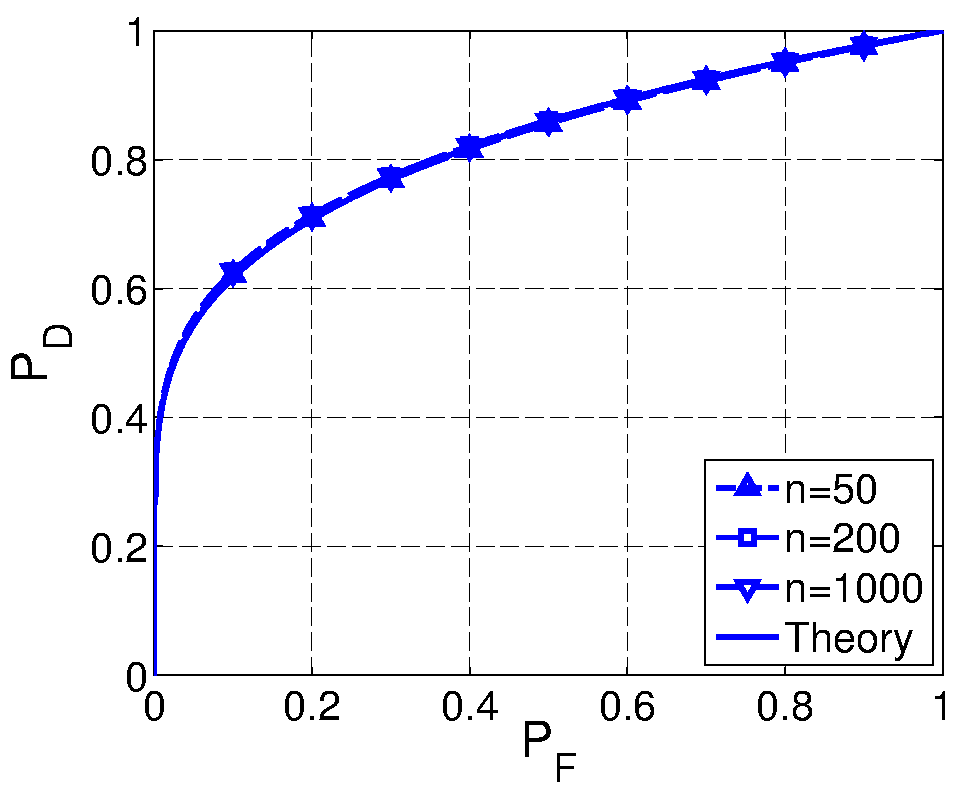
\includegraphics[width=\figwidth]{figures/stoch_n_effect1.pdf}
\label{fig:stoch_n_effect1}
}
\subfigure[$k=4$, $c=10$]{
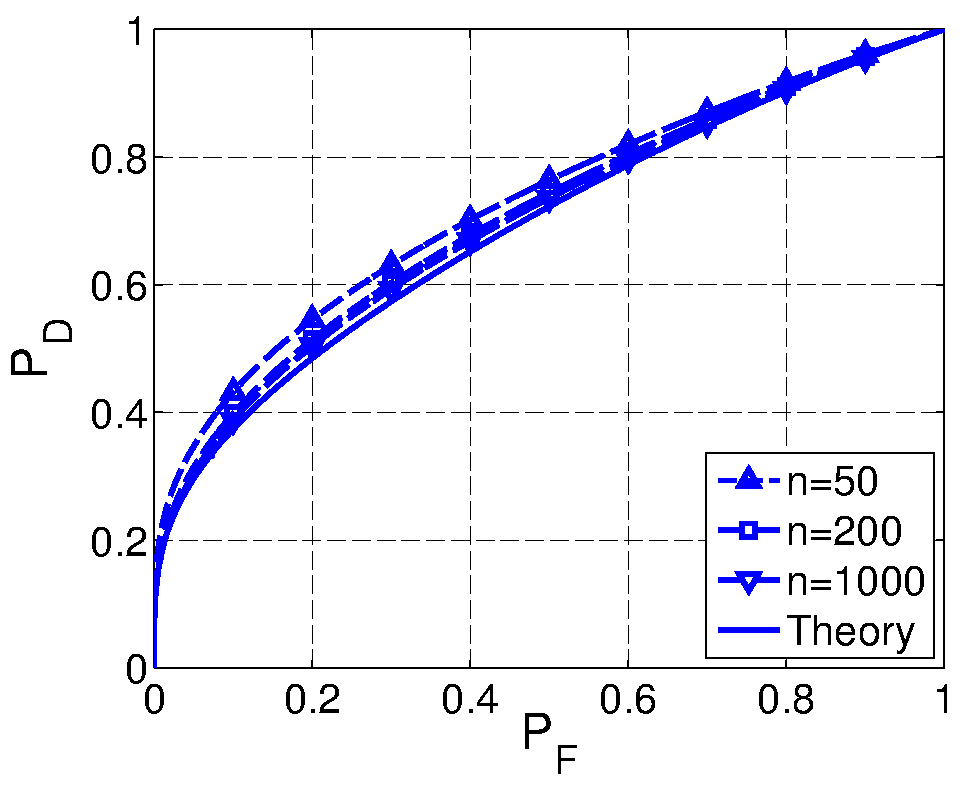
\includegraphics[width=\figwidth]{figures/stoch_n_effect4.pdf}
\label{fig:stoch_n_effect4}
}
\vspace{-0.1in}
\caption{Empirical and theoretical ROC curves for the stochastic plug-in detector. Empirical ROC curves were simulated using $10000$ test samples and averaged over 50 trials using algorithms 2 and 4 of \cite{fawcett2006introduction}. (a) $\Sigma=\diag(10,2)$, $c=1$, $\widehat{k}=k=2$ so that $\keff=2$. (b) $\Sigma=\diag(10,2,0.5,0.1)$, $c=10$, $\widehat{k}=k=4$ so that $\keff=1$. Each figure plots empirical ROC curves for $n=50,200,1000$. Theoretical ROC curves were computed as described in Section \ref{sec:roc_theory}. As $n$ increases, the empirical ROC curves approach the theoretically predicted one. However, this convergence is slower for larger $k$ and $c$.}
\vspace{-0.3in}
\end{figure}

The theoretical ROC curve predictions for the plug-in and RMT detectors rely on the asymptotic approximations that ignore finite $n$ and $m$ correction terms. To examine the validity of the asymptotic approximations (Propositions \ref{th:angles} and \ref{th:eigvals_rmt}, Theorem \ref{th:other angles}, and Corollary \ref{corr:matrix}) and the rate of convergence, we consider two different settings for the stochastic plug-in detector. Figures \ref{fig:stoch_n_effect1}-\ref{fig:stoch_n_effect4} plot three empirical ROC curves for $n=50,200,1000$ as well as the theoretically predicted plug-in ROC curve. Each figure uses different values of $k$ and $c$ but in each case, $\widehat{k}=k$.

For both figures, as $n$ increases, the empirical ROC curves approach the theoretical prediction, attesting to the asymptotic convergence of the RMT approximations. Analyzing the rate of convergence (which we conjecture to be $n^{1/2}$ for fixed $k$ and $c$) is an important open problem that we shall tackle in future work. As evident in Figures \ref{fig:stoch_n_effect1}-\ref{fig:stoch_n_effect4} the values of $k$ and $c$ play an important roll in the convergence of the empirical ROC curves. For the larger value of $k$ and $c$ (corresponding to the sample starved regime where the amount of training data is smaller than the system dimensionality i.e. $n>m$) the convergence is also slower. We see that for larger $k$ and $c$, when $n$ is small the empirical ROC curve is not well approximated by the asymptotic theoretical predictions. However, as $n$ increases, the deviation of the empirically generated ROC curve from the theoretically predicted one decreases. Claim \ref{th:other angles} suggests that the off diagonal terms of $\widehat{U}^HU$ asymptotically tend to zero. However, in the finite $n$ and $m$ case these terms are $O(1/\sqrt{n})$ and thus not identically zero. For larger rank systems (increased $k$), there are more of these non-identically-zero terms that worsen the approximation quality for fixed, relatively small $n$. As $n$ increases, this bias vanishes.

\begin{figure}
\centering
\subfigure[Stochastic]{
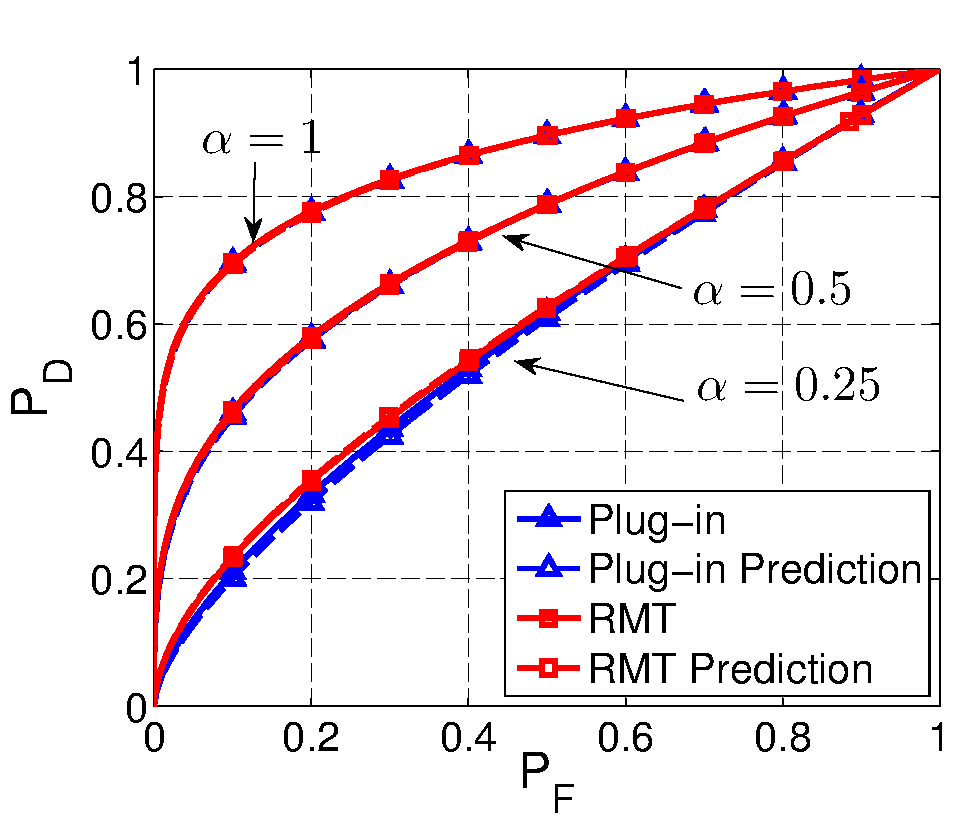
\includegraphics[width=\figwidth]{figures/stoch_roc_pred.pdf}
\label{fig:stoch_roc_pred}
}
\subfigure[Deterministic]{
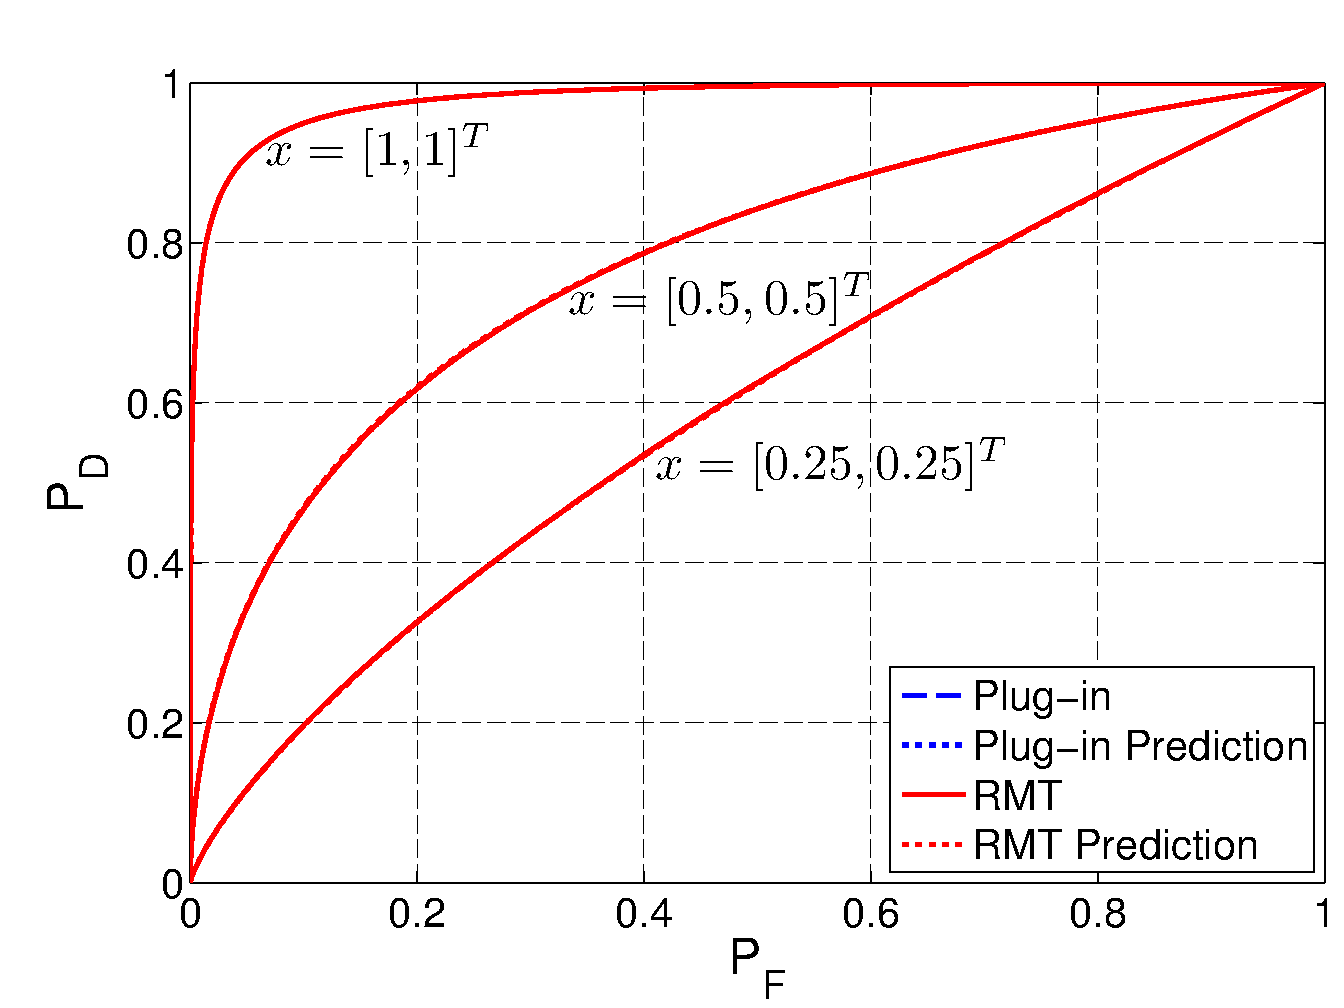
\includegraphics[width=\figwidth]{figures/determ_roc_pred.pdf}
\label{fig:determ_roc_pred}
}
\vspace{-0.1in}
\caption{Empirical and theoretical ROC curves for the plug-in and RMT detectors. Empirical ROC curves were simulated using $10000$ test vectors and averaged over 100 trials with $n=1000$, $m=500$, and $\Sigma =\alpha\diag\left(10,5\right)$. The theoretical ROC curves were computed as described in Section \ref{sec:roc_theory}. (a) Stochastic testing setting. Results are plotted for $\alpha=1,0.5,0.25$. For $\alpha=1$ and $\alpha=0.5$, $\widehat{k}=k=k_\text{eff}=2$ by (\ref{eq:keff}). For $\alpha=0.25$, $k_\text{eff}=1$.Since $\widehat{k} > k_{\text{eff}}$ when $\alpha=0.25$, we observe a performance gain when using the RMT detector. (b) Deterministic testing setting. Results are plotted for $\alpha=1$ so that $\keff=2$. Three values of the deterministic signal vector were used: $x=[1,1]^T$, $x=[0.5,0.5]^T$, and $x=[0.25,0.25]^T$. The resulting ROC curves depend on the choice of $x$, however, since $\widehat{k} = k_{\text{eff}}$, the plug-in and RMT detector achieve the same performance for all $x$. For both the stochastic and deterministic detectors, the theoretically predicted ROC curves match the empirical ROC curves, reflecting the accuracy of Corollary \ref{corr:matrix} and the Lugannani-Rice formula.}
\vspace{-0.3in}
\end{figure}

The ROC predictions developed in Section \ref{sec:roc_theory} also depend on parameters such as $\Sigma$ and the deterministic vector $x$. To test the accuracy of the ROC predictions with respect to these parameters, we consider a setting where $\widehat{k}=k = 2$. Figure \ref{fig:stoch_roc_pred} plots empirical and theoretical ROC curves for the plug-in and RMT stochastic detectors for $\Sigma=\alpha\diag(10,5)$ for three choices of $\alpha$. As intuition suggests, smaller values of $\Sigma$ decrease the performance for both the plug-in and RMT detectors. For each choice of $\alpha$, the empirical ROC curves match the ROC predictions that rely on random matrix theoretic approximations presented in Section \ref{sec:rmt}. Using $\alpha=1$ or $\alpha=0.5$ results in $\keff=k=\widehat{k}=2$ but using $\alpha=0.25$ results in $k_\text{eff}=1$. As $\widehat{k}>k_\text{eff}$ for this last case, the plug-in detector realizes a performance loss compared to the RMT detector.

In the deterministic setting, $x$ is an additional parameter that affects detector performance. Figure \ref{fig:determ_roc_pred} plots empirical and theoretical ROC curves for the plug-in and RMT deterministic detectors for $\Sigma=\diag(10,5)$ for three choices of the deterministic test vector $x$. Larger values of $|x|$ result in better detector performance but for each choice of $x$, the theoretically predicted ROC curves match their empirical counterparts. As $x$ does not affect the value of $k_\text{eff}=\widehat{k}=k=2$, the plug-in and RMT detectors achieve the same performance because they have identical statistics. For both test vector models, the theoretical ROC curves match the empirical ROC curves thereby validating the accuracy of the random matrix theoretic approximations employed and the accuracy of the saddlepoint approximation to the c.d.f. used in the stochastic derivation. 

\subsection{Effect of the Number of Training Samples}

\begin{figure}
\centering
\subfigure[$m=5000$]{
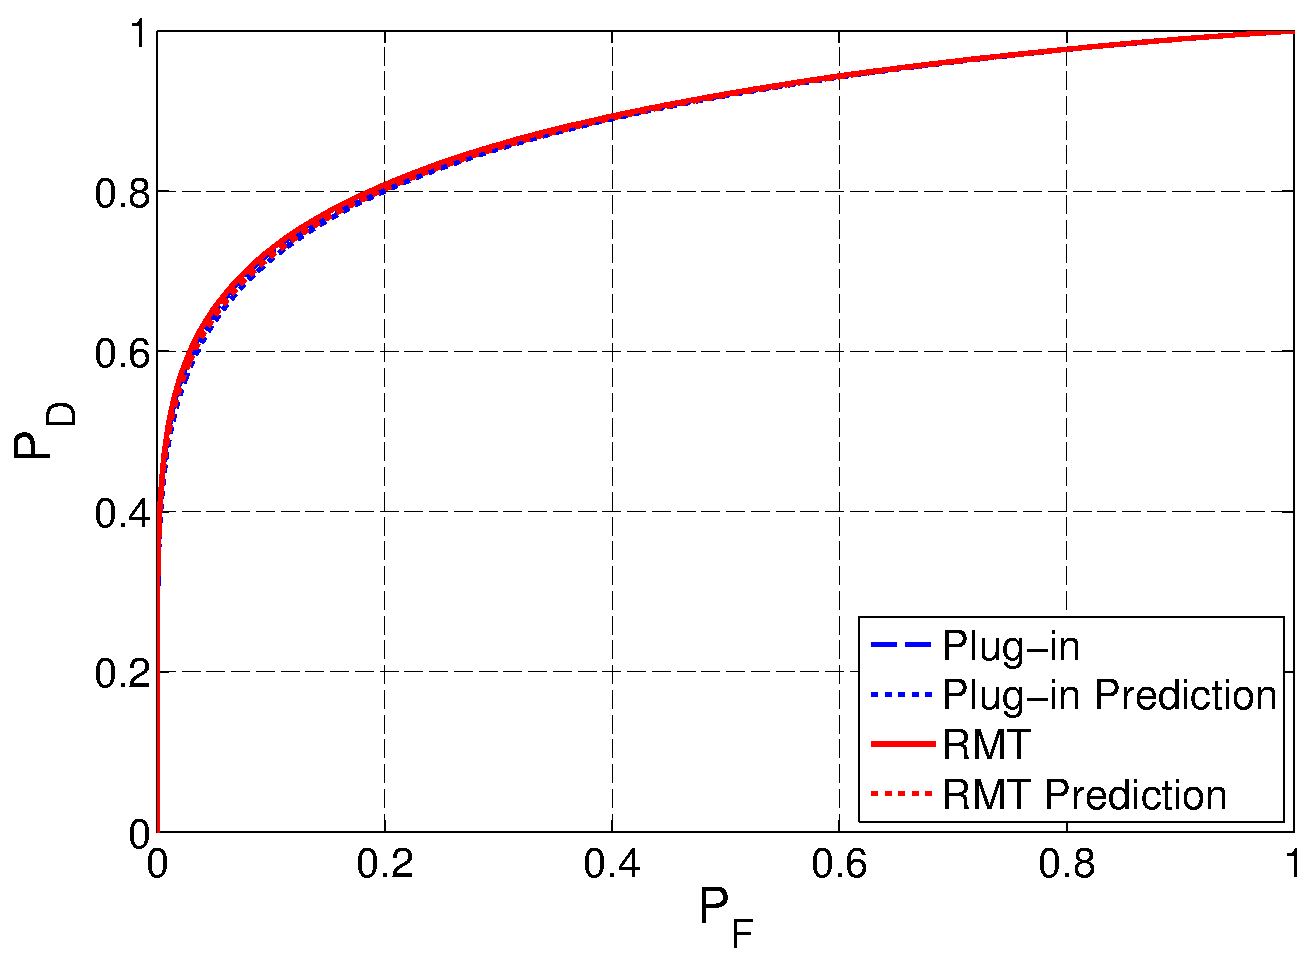
\includegraphics[width=\figwidth]{figures/stoch_m_large.pdf}
\label{fig:stoch_m_large}
}
\subfigure[$m=250$]{
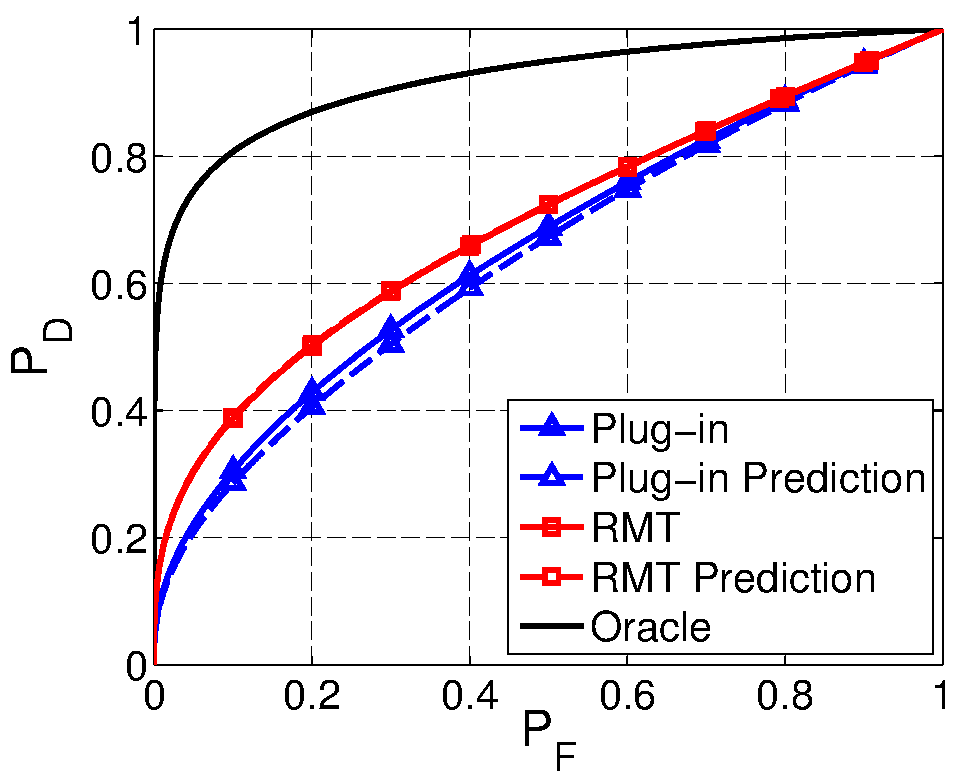
\includegraphics[width=\figwidth]{figures/stoch_m_small.pdf}
\label{fig:stoch_m_small}
}
\vspace{-0.1in}
\caption{Empirical and theoretical ROC curves for the plug-in and RMT stochastic detectors. Empirical ROC curves were computed with 10000 test samples and averaged over 100 trials. Here, $n=5000$, $\widehat{k}=k=4$ and $\Sigma = \diag({\bf{10,3,2.5,2}})$. The empirical oracle ROC curve is provided for relative comparison purposes. (a) $m=5000$ so that $c=1$ and $k_\text{eff}=\widehat{k}=4$. The plug-in and RMT detectors achieve relatively the same performance. (b) $m=250$ so that $c=20$ and $\keff=1<\widehat{k}=4$. The RMT detector avoids some of the performance loss realized by the plug-in detector. As seen in Section \ref{sec:std_detecs}, limited training samples degrades detector performance. However, the new RMT detector does not suffer as badly as the plug-in detector because it accounts for subspace estimation errors due to finite training data. The disagreement between the theoretical and empirical ROC curves is attributed to finite dimensionality.}
\label{fig:stoch_m_effect}
\vspace{-0.3in}
\end{figure}

We saw in Section \ref{sec:training_effect} that finite training data degraded the performance of the plug-in detector relative to that of the oracle detector. The analysis of Section \ref{sec:rmt} mathematically justifies this observation showing that, for a fixed $\Sigma$, the number of training samples, $m$, directly affects $k_\text{eff}$ via (\ref{eq:keff}). While the plug-in detector ignores this analysis, we derived a new RMT detector that accounts for subspace estimation errors due to finite training data. By only using the $\keff$ informative signal subspace components, we hope that the RMT detector will avoid some of the performance loss associated with the plug-in detector. To explore how the number of training samples affects the relative performances of the plug-in and RMT detectors, we first consider the setting where $\widehat{k}=k=4$ with $\Sigma=\diag(10,3,2.5,2)$. 

Figure \ref{fig:stoch_m_large} investigates the performance when $m=n$ so that $c=1$ for
the stochastic setting.  This
choice of $m$ results in $k_\text{eff}=\widehat{k}=4$. As expected, the plug-in and RMT
detectors achieve relatively the same performance because $\widehat{k}=\keff$. A similar
phenomenon occurs in the deterministic setting. Figure
\ref{fig:stoch_m_small} chooses $20m=n$ so that $c=20$ and $k_\text{eff}=1$ for the
stochastic settings. This corresponds to the sample starved regime where $m<n$. In this
second experiment, the plug-in detector becomes suboptimal because it uses $4=\widehat{k}
> k_\text{eff}=1$ subspace components. A similar phenomenon occurs in the deterministic
setting. Whenever $k_\text{eff}<\widehat{k}$ the RMT detectors avoid some of the performance loss (compared to the oracle detectors) realized by the plug-in detectors. We could have observed this same effect by instead varying $\Sigma$ as both of these quantities drive the value of $k_\text{eff}$. The disagreement between the theoretical and empirical stochastic ROC curves for the plug-in detector is attributed to the finite $n$ and $m$ correction terms, which we have discussed previously.

Figure \ref{fig:stoch_m_effect} shows that the number of training samples helps to drive the performance of matched subspace detectors. In Section \ref{sec:std_detecs}, we mathematically defined the performance loss of a detector relative to its oracle detector as $\epsilon$ in (\ref{eq:epsilon}) and empirically plotted the number of training samples needed to achieve a desired performance loss for the stochastic plug-in detector in Figure \ref{fig:epsilon_graph}. Figures \ref{fig:stoch_theory_epsilon} and \ref{fig:determ_theory_epsilon} theoretically plot this same curve for the plug-in and RMT detectors for each testing setting, respectively.

These figures show that when $\keff<\widehat{k}$, the RMT detector achieves a much smaller performance loss for a fixed number of training samples. Put another way, to achieve the same performance loss, the RMT detectors need a significantly less number of training samples when $\keff<\widehat{k}$. Figure \ref{fig:stoch_theory_epsilon} shows that the stochastic detectors can achieve an arbitrarily small performance loss given a particularly large number of training samples. However, Figure \ref{fig:determ_theory_epsilon} shows that there is a performance loss limit for the deterministic detectors. As discussed in Section \ref{sec:std_detecs}, this arises because the oracle deterministic detector assumes that $x$ is known. As $m\to\infty$, $\widehat{U}\to U$ and $\widehat{\Sigma}\to\Sigma$, however, the plug-in detector's estimate of $\widehat{x}$ still depends on the noisy observed data $y$. Therefore, unlike the stochastic detectors that can achieve an arbitrarily small performance loss, the deterministic plug-in and RMT detectors can never achieve the same performance as the deterministic oracle detector.

\begin{comment}
\begin{figure}
\centering
\subfigure[$m=5000$]{
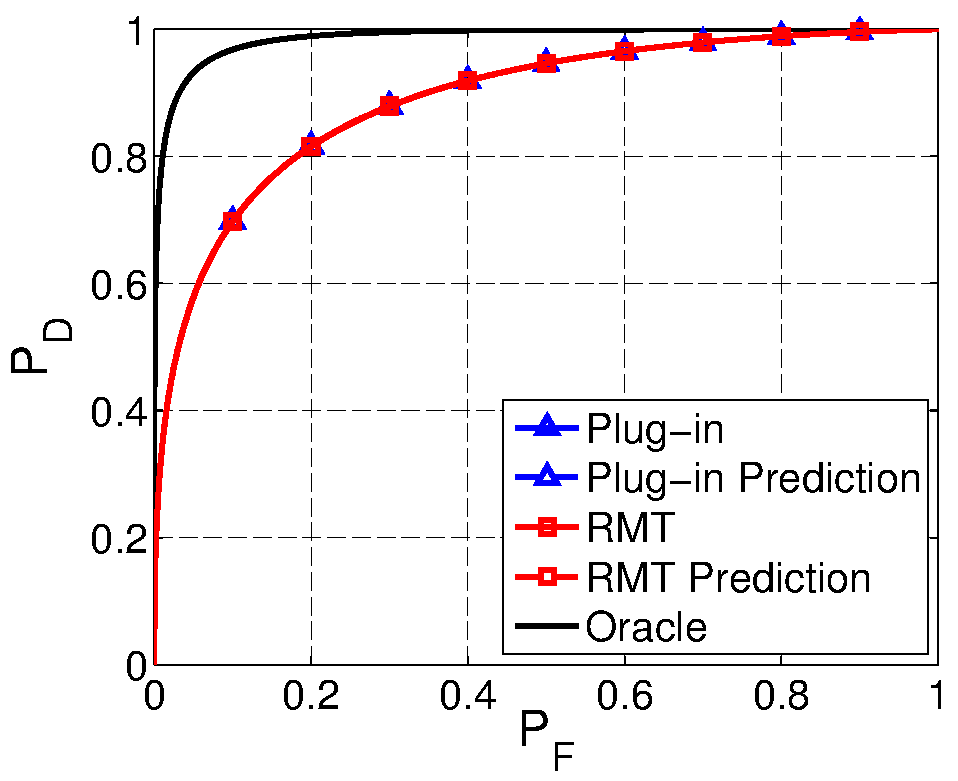
\includegraphics[width=\figwidth]{figures/determ_m_large.pdf}
\label{fig:determ_m_large}
}
\subfigure[$m=250$]{
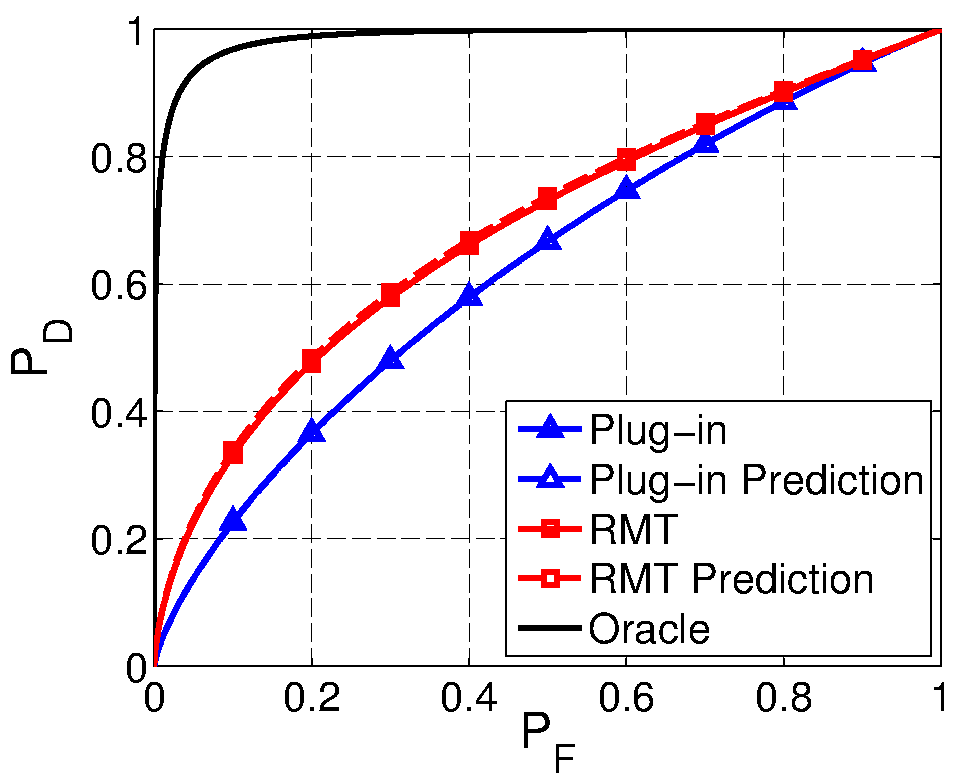
\includegraphics[width=\figwidth]{figures/determ_m_small.pdf}
\label{fig:determ_m_small}
}
\vspace{-0.1in}
\caption{Analogous figures to Figures \ref{fig:stoch_m_large} and \ref{fig:stoch_m_small} for the deterministic detectors when $x=0.75\times[1,1,1,1]^T$. When $\keff<\widehat{k}$ we see that the RMT detector avoids some of the performance loss of the plug-in detector due to finite training data.}
\label{fig:determ_m_effect}
\vspace{-0.2in}
\end{figure}
\end{comment}

\begin{figure}
\centering
\subfigure[Stochastic]{
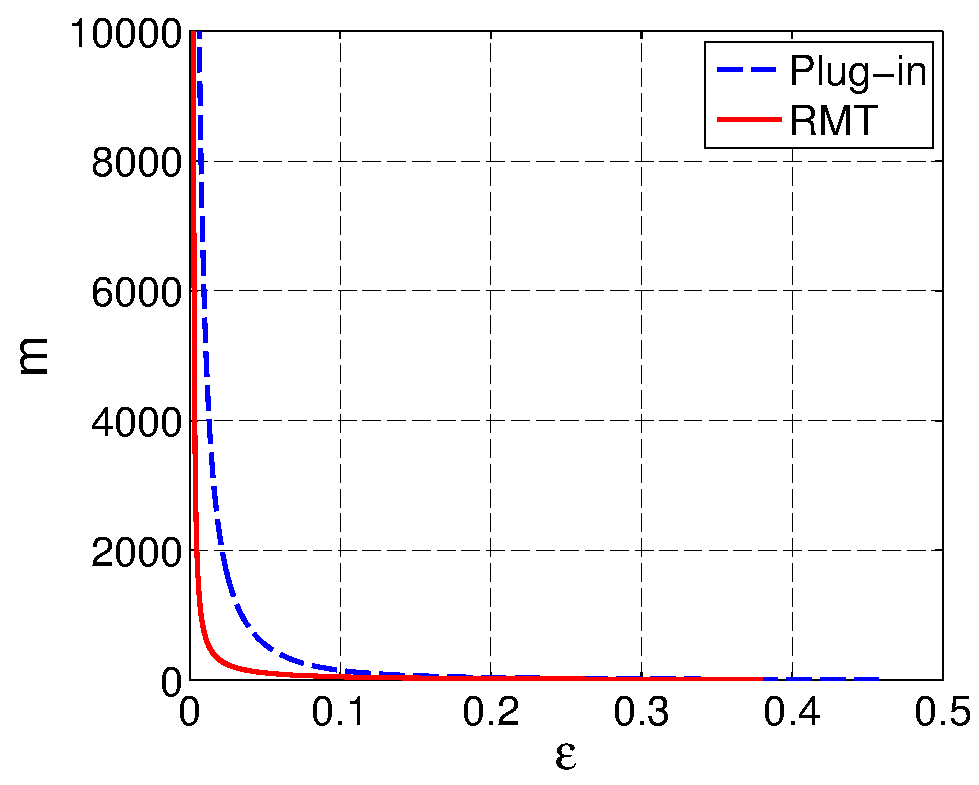
\includegraphics[width=\figwidth]{figures/stoch_theory_epsilon_graph.pdf}
\label{fig:stoch_theory_epsilon}
}
\subfigure[Deterministic]{
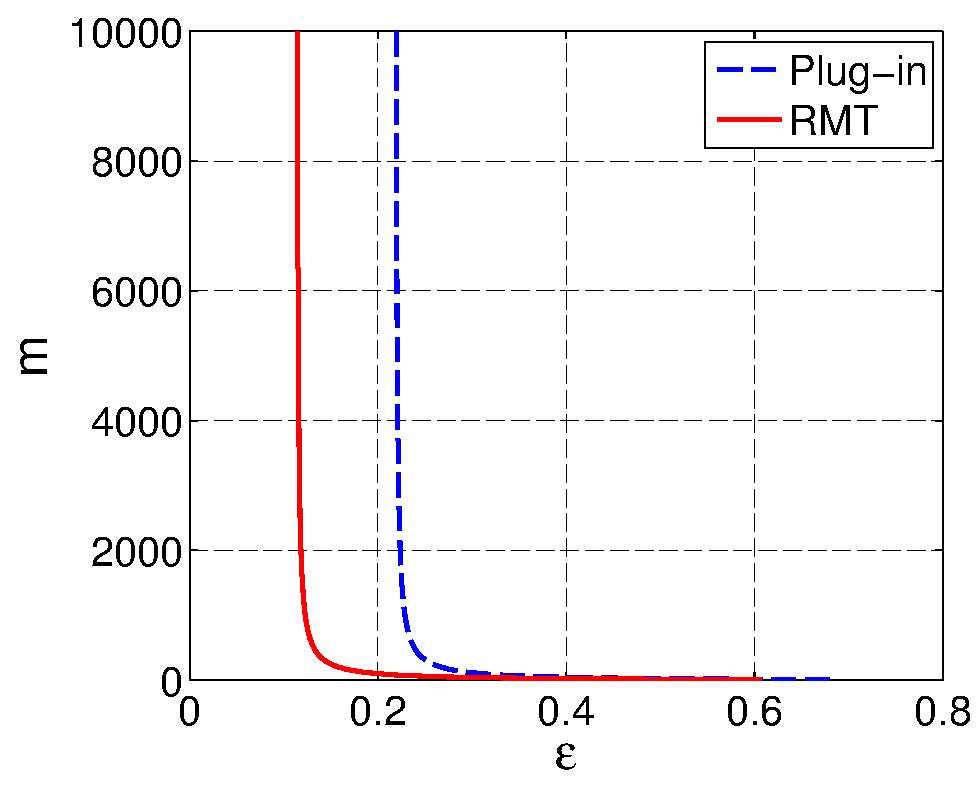
\includegraphics[width=\figwidth]{figures/determ_theory_epsilon_graph.pdf}
\label{fig:determ_theory_epsilon}
}
\vspace{-0.1in}
\caption{Theoretically determined number of training samples, $m$, needed to achieve a desired performance loss, $\epsilon$, as defined in (\ref{eq:epsilon}). The required false alarm rate is $P_F=0.1$ with $n=200$, $\Sigma = \diag(10,0.1)$, and $\widehat{k}=k=2$. (a) Results for the stochastic detectors. We see that for a given $\epsilon$, the new RMT detector requires less training samples. (b) Results for the deterministic detectors when $x=[0.75,0.75]^T$. Again, for a given $\epsilon$, the new RMT detector requires less training samples. In the deterministic setting, the limiting performance loss is different (and non-zero) for the plug-in and RMT detectors. This arises in estimation errors of $x$ in the GLRT.}
\label{fig:epsilon_combined}
\end{figure}

\subsection{Effect of $\widehat{k}$}
\begin{figure}
\centering
%\subfigure[Stochastic]{
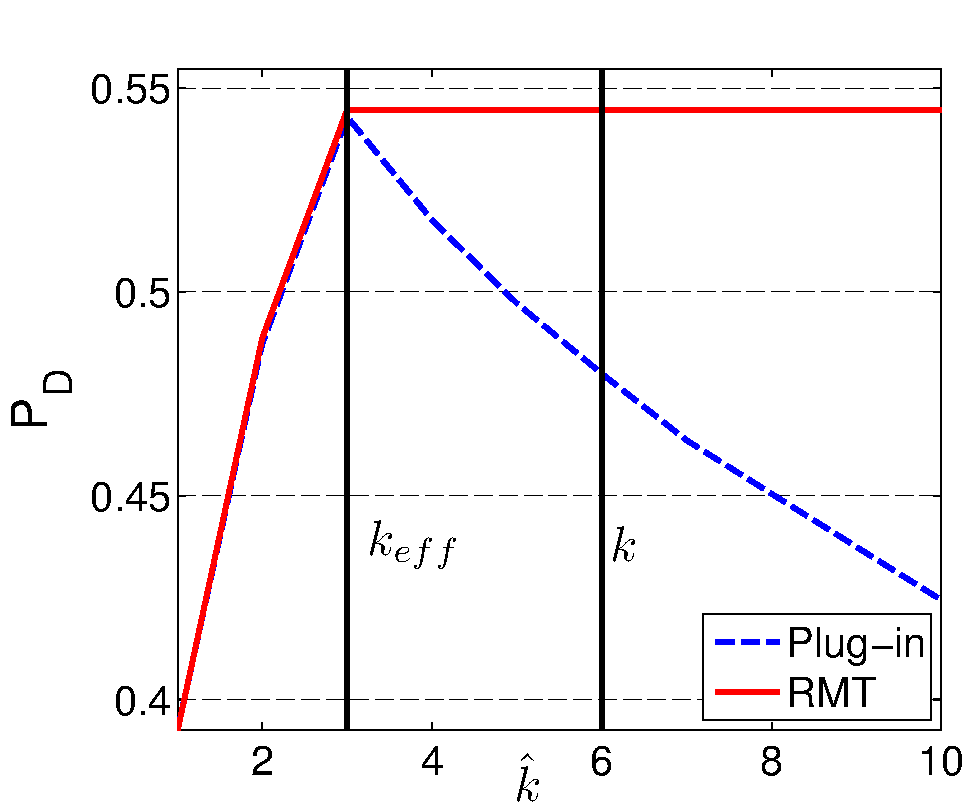
\includegraphics[width=\figwidth]{figures/stoch_khat_graph.pdf}
\label{fig:stoch_khat}
%}
%\subfigure[Deterministic]{
%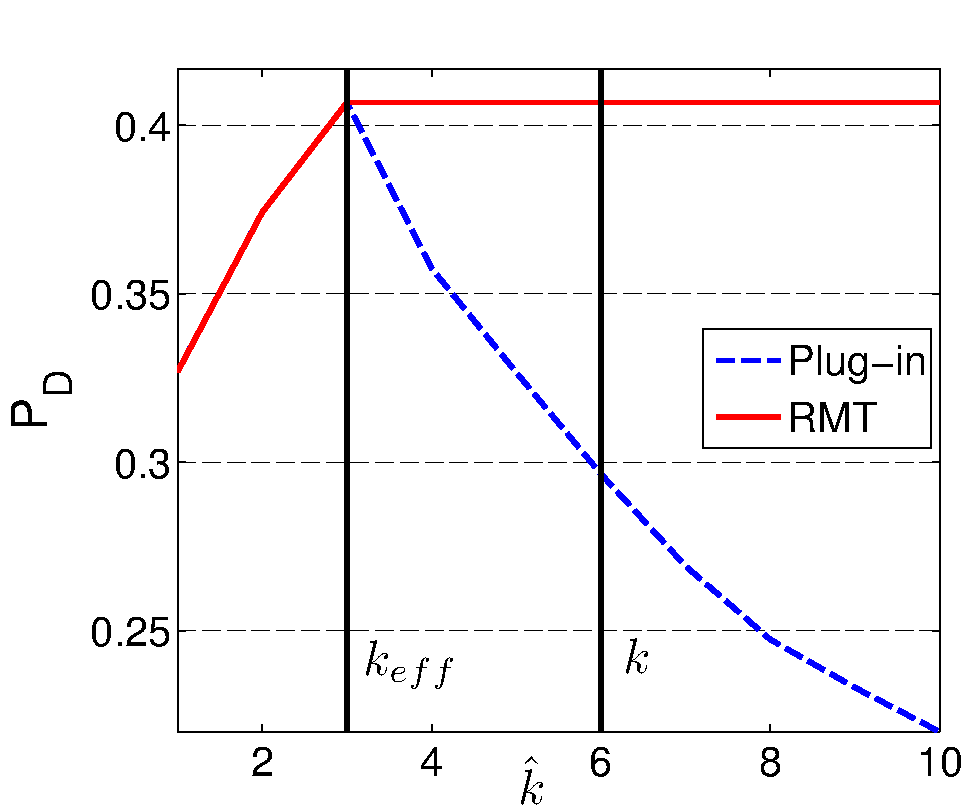
\includegraphics[width=\figwidth]{figures/determ_khat_graph.pdf}
%\label{fig:determ_khat}
%}
\vspace{-0.1in}
\caption{Empirical exploration of the achieved probability of detection, $P_D$, for a
  fixed probability of false alarm, $P_F=0.01$, for various $\widehat{k}$. Empirical ROC
  curves were computed using 10000 test samples and averaged over 100 trials with
  $n=1000$, $m=500$, and $\Sigma = \diag({\bf{10,5,4}},0.75,0.5,0.25)$ so that
  $k_{\text{eff}}=3$. Results for the stochastic detectors. The optimal $\widehat{k}$ resulting in the largest $P_D$ is not the true $k$, but rather $k_\text{eff}$.} %(b) Results for the deterministic detectors using $x=0.75\times[1,1,1,1,1,1]^T$. In both test settings, the optimal $\widehat{k}$ resulting in the largest $P_D$ is not the true $k$, but rather $k_\text{eff}$.}
\label{fig:khat_graphs}
\vspace{-0.3in}
\end{figure}

We discussed in Section \ref{sec:param_estim} that we are given a dimension estimate
$\widehat{k}$ when deriving our detector. From our perspective, we don't know how
$\widehat{k}$ was estimated (possibly from the training data or by a domain expert) but
simply use it when forming our subspace and signal covariance estimates. Figure
\ref{fig:khat_graphs} empirically examines the performance of the plug-in and RMT detectors
as a function of $\widehat{k}$ for the stochastic setting. A similar phenomenon arises in
the deterministic setting. Here, we relax the constraint that $\widehat{k}\geq k$. The figures plot the achieved probability of detection for a constant false alarm rate of $0.01$. The result confirms that $k_\text{eff}$ is the optimal choice for $\widehat{k}$. When the plug-in detectors use $\widehat{k} = k_\text{eff}$ they achieve an equivalent performance as that of the RMT detector.

Setting $\widehat{k} < \keff$ drastically degrades performance for all detectors. In this regime, the plug-in and RMT detectors realize the same ROC performance, demonstrating that quantification and exploitation of the subspace estimation accuracy ($|\langle u_i,\widehat{u}_i\rangle |^2_{\text{rmt}}$ and $\sigma_{i_\text{rmt}}^2$), while useful in ROC performance prediction, does \textit{not} noticeably enhance detection performance. When $\widehat{k} > k_\text{eff}$, the performances of the plug-in detectors degrade while those of the RMT detectors are stable as if $\widehat{k}=k_\text{eff}$. In other words, we do not pay a price for overestimating the subspace dimension with the RMT detectors. This makes sense (and is slightly contrived) because the RMT detectors will only sum to a maximum of $k_\text{eff}$ indices as evident in (\ref{eq:optimal_stat_stoch}) and (\ref{eq:optimal_stat_determ}). In many applications, practitioners might employ the ``play-it-safe'' approach and set $\widehat{k}$ to be significantly greater than $k_\text{eff}$. The performance loss caused by adding each uninformative subspace, as seen in Figure \ref{fig:khat_graphs}, constitutes evidence to the assertion that overestimating the signal subspace dimension is a bad idea. When $k_\text{eff} < k$, even perfectly estimating the subspace dimension (i.e. setting $\widehat{k} = k$) is suboptimal.
